\documentclass[pdf]{beamer}
\usepackage[latin1]{inputenc}
\usepackage{multirow}
\usetheme{Goettingen} %Warsaw
\usecolortheme{seagull}

\usepackage{movie15}

\begin{document}

\title[Introduction to Sequencing]{Introduction to Sequencing}
\subtitle{BCB 504: Applied Bioinformatics\\}
\author[Matt Settles]{Matt Settles}
\institute{University of Idaho\\ Bioinformatics and Computational Biology Program}
\date{\today}


%% Title page
\begin{frame}[plain]
  \titlepage
\end{frame}


%% Outline
\begin{frame}[plain] 
  \frametitle{Outline}
  \tableofcontents
\end{frame}

\section{History}
\begin{frame}
  \frametitle{Evolution of DNA Sequencing}
  {\footnotesize Jan - 2012: \$0.09 per Megabase, \$7,950 per Genome (30x coverage)}
  \begin{center}
  \begin{figure}
    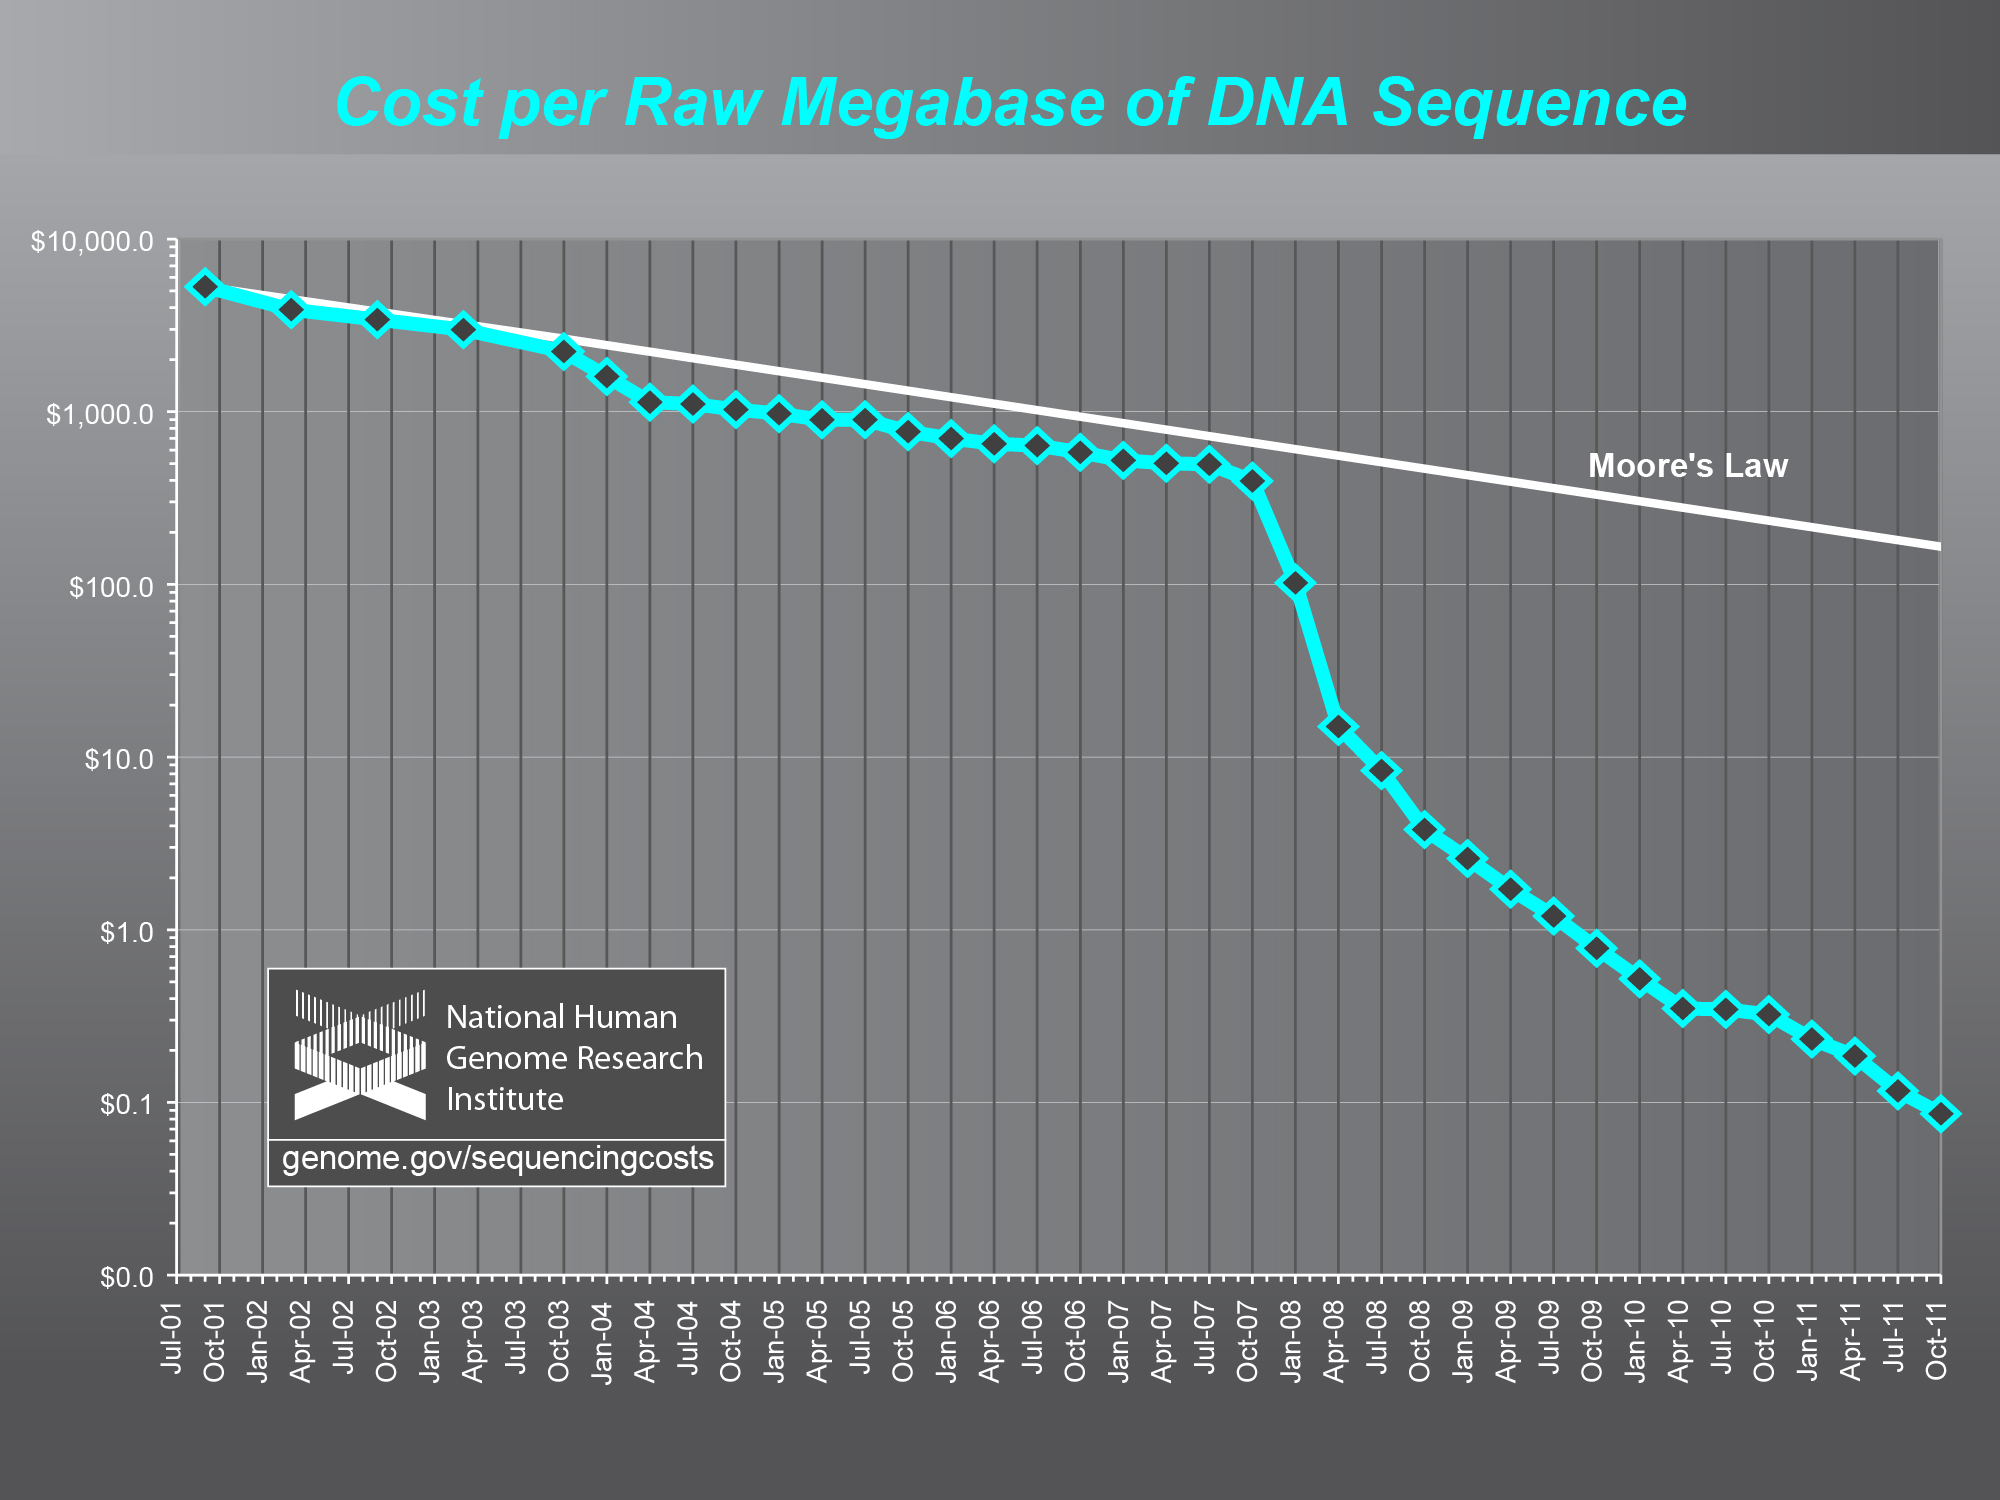
\includegraphics[scale=0.4]{cost_per_megabase.jpg}
  \end{figure}
  \end{center}
\end{frame}

\section{Roche 454 Pyrosequencing}

\begin{frame}
  \frametitle{Roche 454 Workflow}
  \begin{itemize}
  \item Library Construction
  \item QA - Library Quantification (Titration)
  \item emulsion PCR (emPCR)
  \item Picotiter Plate Loading
  \item Sequencing
  \item Image extraction
  \item Flowgram extraction
  \end{itemize}
\end{frame}

\begin{frame}
  \frametitle{Roche 454 Workflow Video}
  \begin{center}
  \href{http://www.youtube.com/watch?feature=player_detailpage&v=bFNjxKHP8Jc}{454 Video}
  \end{center}  
\end{frame}

\begin{frame}
  \frametitle{Roche 454 Flowgrams}
  \begin{center}
    \begin{figure}
    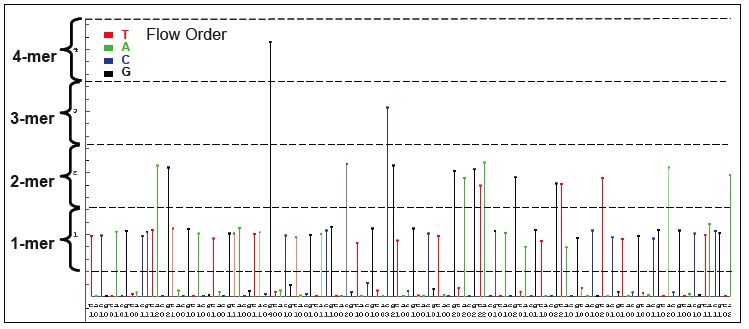
\includegraphics[scale=0.35]{Flowgram.jpg}
  \end{figure}
  \end{center}
\end{frame}

\section{Illumina Solexa}

\begin{frame}
  \frametitle{Illumina Workflow}
  \begin{itemize}
  \item Library Construction
  \item Cluster Generation
  \item Sequencing
  \item image extraction
  \end{itemize}
\end{frame}
  
\begin{frame}
  \frametitle{Illumina Workflow Video}
  \begin{center}
  \href{http://www.youtube.com/watch?NR=1&feature=endscreen&v=l99aKKHcxC4}{Illumina Video}
  \end{center}
\end{frame} 

\section{Sequence Data}

\begin{frame}
  \frametitle{Illumina Read Naming Conventions}
  \begin{small}
  @EAS139:136:FC706VJ:2:2104:15343:197393 1:Y:18:ATCACG\\
  \end{small}  
  \begin{description}
  \item[EAS139]	the unique instrument name
  \item[136]	the run id
  \item[FC706VJ]	the flowcell id
  \item[2]	flowcell lane
  \item[2104]	tile number within the flowcell lane
  \item[15343]	'x'-coordinate of the cluster within the tile
  \item[197393]	'y'-coordinate of the cluster within the tile
  \item[1]	the member of a pair, 1 or 2 (paired-end or mate-pair reads only)
  \item[Y]	Y if the read fails filter (read is bad), N otherwise
  \item[18]	0 when none of the control bits are on, otherwise it is an even     number
  \item[ATCACG]	index sequence
  \end{description}
\end{frame}

\begin{frame}
  \frametitle{454 Read Naming Convections}
  $>$EBO6PME01EGNVK
  \begin{description}
  \item[Timestamp] EB06PM
  \item[Randomized ] E
  \item[Plate Region] 01
  \item[X,Y coord] EGNVK
  \end{description}
  The timestamp, hash character and X,Y location use a base-36 encoding (where values 0-25 are the letters 'A'-'Z' and the values 26-35 are the digits '0'-'9'). An accession thus consists only of letters and digits, and is case-insensitive. 
\end{frame}
   
\begin{frame}
  \frametitle{fasta,qual and fastq files}
  \begin{itemize}
  \item fasta files\\%
  $>$sequence1\\
  ACCCATGATTTGCGA
  \item qual files\\%
  $>$sequence1\\
  40 40 39 39 40 39 40 40 40 40 20 20 36 39 39
  \item fastq files\\%
  $@$sequence1\\
  ACCCATGATTTGCGA\\
  $+$\\
  IIHHIHIIII55EHH
  \end{itemize}
\end{frame}

\begin{frame}
  \frametitle{phred scores}
$Q = -10log_{10}P$
\begin{center}
\begin{tabular}{|l|l|l|}
\hline
Phred & Probability &	Base call \\
Quality Score	& of incorrect  & accuracy \\
 & base call & \\
\hline
10	&	1 in 10	&	$90\%$\\
20	&	1 in 100 &	$99\%$\\
30	&	1 in 1000	&	$99.9\%$\\
40	&	1 in 10000	&	$99.99\%$\\
\hline
\end{tabular}
\end{center}
\end{frame}
% fasta
% qual
% fastq
%% quality scores
\begin{frame}
  \frametitle{phred score conversion}
$Q_{sanger} = -10log_{10}P$ - based on probability (aka phred)
\\

$Q_{solexa} = -10log_{10}\frac{P}{1-P}$ - based on odds
\begin{center}
\begin{tabular}{ l l l }
S - Sanger        &Phred+33,  &raw reads typically (0, 40) \\
X - Solexa        &Solexa+64, &raw reads typically (-5, 40) \\
I - Illumina 1.3+ &Phred+64,  &raw reads typically (0, 40) \\
J - Illumina 1.5+ &Phred+64,  &raw reads typically (3, 40) \\
L - Illumina 1.8+ &Phred+33,  &raw reads typically (0, 41) \\
\end{tabular}
\end{center}
\end{frame} 


\section{Library Preparation}
\begin{frame}
 \frametitle{Library Preparation types}
 \begin{itemize}
 \item Shotgun - randomly fragmented DNA (100bp - 1kb) 
 \item RNA - Random nanomers or 3' bias
 \item Amplicons
 \item Paired end / Mate pair
 \end{itemize}
\end{frame} 

\section{Other sequencing technologies}
\begin{frame}
  \frametitle{Ion Torrent Workflow Video}
  \begin{center}
  \href{http://www.youtube.com/watch?v=yVf2295JqUg}{Ion Torrent Video}
  \end{center}
\end{frame} 


\begin{frame}
  \frametitle{Pacific Biosciences Workflow Video}
  \begin{center}
  \href{http://www.youtube.com/watch?v=NHCJ8PtYCFc&feature=endscreen&NR=1}{Pacific Biosciences Video}
  \end{center}
\end{frame} 


\end{document}

